\documentclass[10pt]{article}
\usepackage[margin=18mm]{geometry}
\usepackage{graphicx,booktabs,hyperref}
\usepackage[strings]{underscore}
\setlength{\parindent}{0pt}\setlength{\parskip}{5pt}
\begin{document}
\section*{Fresh fixture generation: 36 frozen cells}

Run fixtures-20261023-01: 36 native commands, 32 public draws each, all
exited zero. There are 1,152 frozen draws in nine parameter cells, each with
prefix, geometric, trace-zero geometric and random bases. Original seed is
20261023; no draws are dropped when a class is absent.

\begin{center}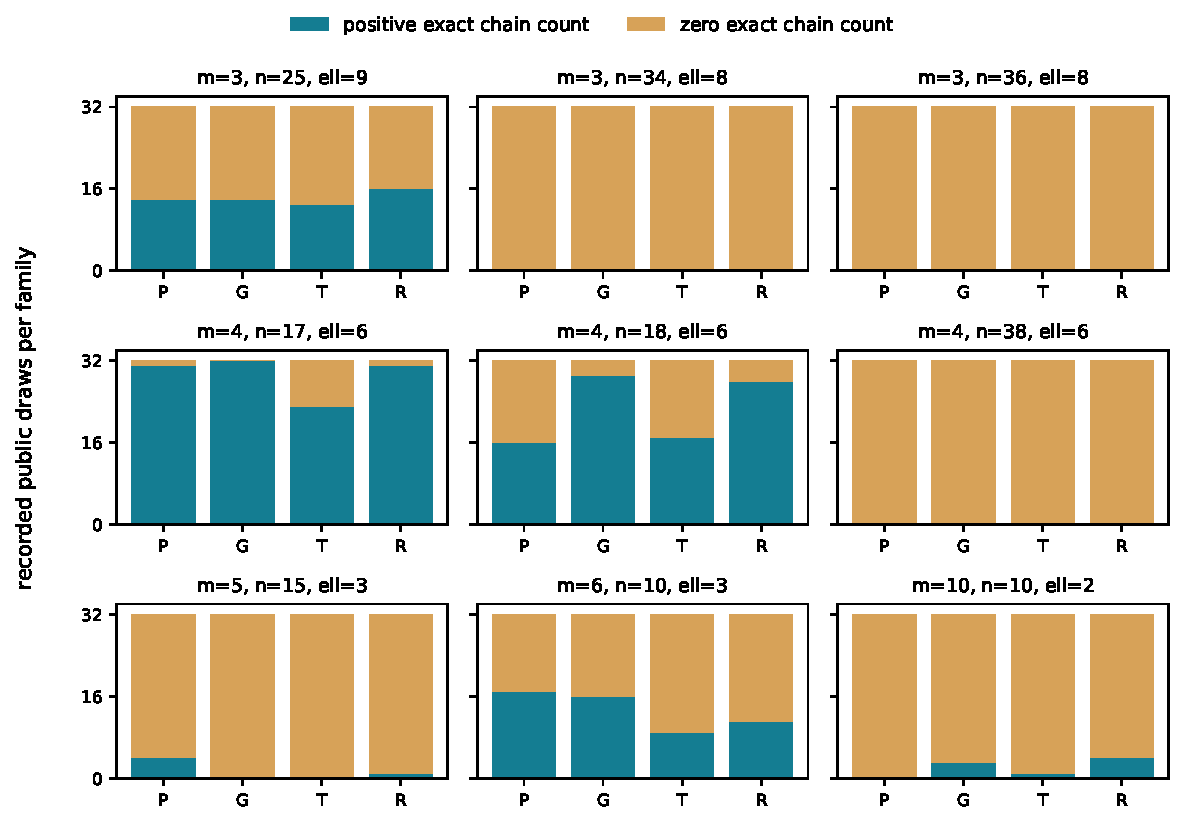
\includegraphics[width=\linewidth]{fixture-outcomes.pdf}\end{center}

P=prefix, G=geometric, T=trace-zero geometric, R=random. Values are native
recorded counts, not sampled degree measurements or performance comparisons.

The exact algebraic chain counter uses a quadratic Artin--Schreier solve and
meet-in-the-middle at m=3,4, forward dynamic programming for $m>4$. Small-field
controls agree with exhaustive roots and the legacy chain counter. Counts
are not point decompositions or Gröbner results. The larger positive-count
fixtures have not all received independent Boolean-witness replay; their
closure/guess experiments remain open.

The first four zero-count and first three positive-count draws are frozen
per cell/family in inputs/fresh/selection.json; missing classes remain
explicit. Parameter cells include the actual upstream N=58 and N=60
continuations and an N=100 cell. Their generators do not certify a low
solving degree. Limits were 12 GiB and 900 s per native command; L0.

Source: examples/ic_algebraic_followup.rs and exact.rs, built at d67f6085.
Raw rows, commands, input/binary/source hashes and host receipts are in
the fixtures-20261023-01 directory in the evidence archive. The committed
input JSONL files retain field modulus, seed, basis, target, count and
oracle name; their SHA-256 list is inputs/fresh/SHA256SUMS. Native histogram
recomputation and visual values are in report-data.json. No timing or
scaling conclusion follows from this generation run.

\end{document}
